%\appendix 
\refstepcounter{chapter} 
\chapter*{How Long Is the Great Tribulation? The Seventy Sevens of Daniel}\index{Great Tribulation}\index{seventy sevens (Daniel 9)}\index{Daniel} 
\markboth{Appendix~\thechapter\quad How Long Is the Great Tribulation?}%
         {Appendix~\thechapter\quad How Long Is the Great Tribulation?}
%\addcontentsline{toc}{chapter} {\protect\numberline{Appendix~\thechapter} How Long Is the Great Tribulation? The Seventy Sevens of Daniel}
\addcontentsline{toc}{chapter} {\protect\numberline{\thechapter} How Long Is the Great Tribulation? The Seventy Sevens of Daniel}


\section*{A Seven-Year Great Tribulation}\index{Great Tribulation}

The following explanation represents the premillennialist\index{premillennialism} interpretation.

Daniel\index{Daniel} 9 is a key passage for understanding the events of the last days.

\begin{ScriptureBox}

\item[9:24] ``Seventy `sevens' are decreed for your people and your holy city to finish transgression, to put an end to sin, to atone for wickedness, to bring in everlasting righteousness, to seal up vision and prophecy and to anoint the Most Holy Place.''

\item[9:25] ``Know and understand this: From the time the word goes out to restore and rebuild Jerusalem until the Anointed One, the ruler, comes, there will be seven `sevens,' and sixty-two `sevens.' It will be rebuilt with streets and a trench, but in times of trouble.''

\item[9:26] ``After the sixty-two `sevens,' the Anointed One will be put to death and will have nothing. The people of the ruler who will come will destroy the city and the sanctuary. The end will come like a flood: War will continue until the end, and desolations have been decreed.''

\item[9:27] ``He will confirm a covenant with many for one `seven.' In the middle of the `seven' he will put an end to sacrifice and offering. And at the temple he will set up an abomination that causes desolation, until the end that is decreed is poured out on him.''

\end{ScriptureBox}

The angel told Daniel that seventy sevens\index{seventy sevens (Daniel 9)} had been decreed for his people and the holy city\index{holy city} of Jerusalem\index{Jerusalem}.

The underlying Hebrew expression refers to a unit of seven. In this context, it is commonly understood to mean seven years. Thus, seventy sevens\index{seventy sevens (Daniel 9)} amount to \(70 \times 7 = 490\) years.

In the traditional premillennialist\index{premillennialism} interpretation, the seventieth seven is a future seven-year period associated with the Great Tribulation\index{Great Tribulation}.

The first seven sevens (49 years) and the following sixty-two sevens (434 years) are generally understood within this interpretation as having already been fulfilled in history.

\begin{itemize}
\item \textbf{The seven sevens (49 years):} This period is commonly associated with the twentieth year of King Artaxerxes of Persia, around 445 B.C., when he authorized Nehemiah to return and rebuild Jerusalem\index{Jerusalem} (Nehemiah 2:1--8). The period begins with the command to restore and rebuild the city.

\item \textbf{The sixty-two sevens (434 years):} Together with the first seven sevens, this period makes sixty-nine sevens, or 483 years. If calculated using the 360-day year often employed in certain interpretations of biblical prophecy, 483 years amount to approximately 173,880 days. Some interpreters understand this calculation as pointing to the time when Jesus entered Jerusalem\index{Jerusalem} riding on a donkey and was welcomed as King. The words ``the Anointed One will be put to death and will have nothing'' are understood as referring to Christ's crucifixion.\footnote{The following statement, ``The people of the ruler who will come will destroy the city and the sanctuary,'' is commonly understood as referring to the Roman army's conquest of Jerusalem and destruction of the Temple in A.D. 70.}
\end{itemize}

\section*{The Great Tribulation as the Seventieth Seven}\index{Great Tribulation}

Readers may have noticed that, in this interpretation, Daniel\index{Daniel}'s seventy sevens\index{seventy sevens (Daniel 9)} do not follow one another without interruption. The first sixty-nine sevens belong to the past, while the seventieth seven remains in the future. A substantial interval lies between them.

One widely held explanation can be illustrated by the timeline shown in the figure below.

Imagine looking at a mountain range from a distance. Two peaks may appear to rise close together, almost as though they touch. Yet when you draw nearer, you discover a deep valley between them. The Old Testament prophets often saw future events in a similar way. They saw the mountain peaks: the Messiah\index{Messiah}'s suffering, the Messiah's glory\index{glory}, and the judgment\index{judgment} at the end of the age. These events appeared together in their prophetic vision, but the valley between them remained hidden from view. That valley represents the present age of the church.

This phenomenon is often called \emph{prophetic foreshortening}.\footnote{It is also known as ``prophetic telescoping'' or ``prophetic perspective.'' The mountain-peak illustration is one way of describing this feature of biblical prophecy.}

Figure \ref{fig:valley} shows the view. Period \ding{172} represents the 483 years associated with the fulfillment of the first sixty-nine sevens. Period \ding{173} represents the final seven, understood here as the future seven-year Great Tribulation\index{Great Tribulation}. Period \ding{174} represents the valley: the age of grace\index{grace} in which the church is gathered, a mystery not fully revealed to the Old Testament prophets.

{
\begin{figure}[htbp]
    \centering
    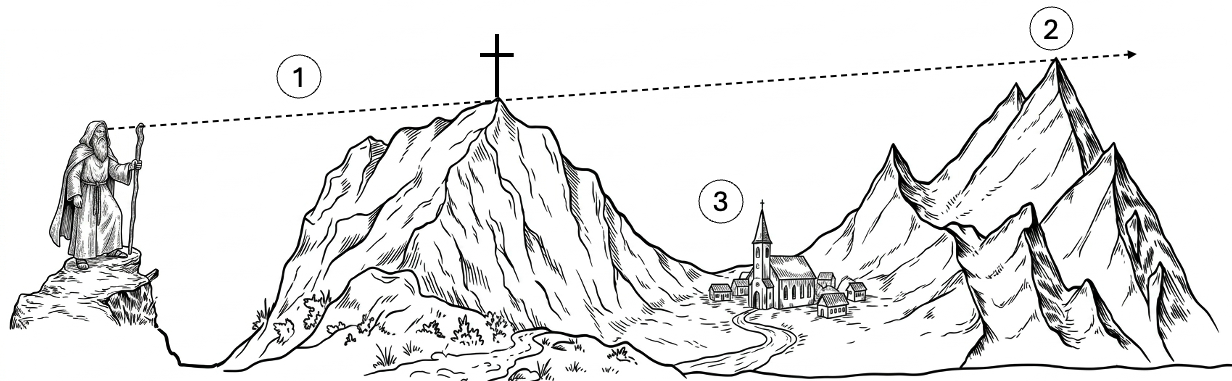
\includegraphics[
        width=1\textwidth,
        trim=0 0 0 0,
        clip]{images/mountain_peak_valley.png}
    \caption{Prophetic Foreshortening}
    \label{fig:valley}
\end{figure}
}

\normalsize

Why was the valley hidden from view?

Paul explains that the church was part of a \textbf{mystery} that had not been fully revealed in earlier generations. Ephesians 3:5 says that this mystery ``has now been revealed by the Spirit to God's holy apostles and prophets.'' Colossians 1:26 describes it as ``the mystery that has been kept hidden for ages and generations, but is now disclosed to the Lord's people.''%
\footnote{A particularly clear example appears when Jesus reads from Isaiah in the synagogue at Nazareth. He reads the words about proclaiming the year of the Lord's favor, then rolls up the scroll and declares, ``Today this scripture is fulfilled in your hearing'' (Luke 4:18--21, NIV). He does not continue to the next phrase in Isaiah 61:2, which speaks of the day of vengeance of our God. In Isaiah's prophecy, these two phrases stand close together. In their historical fulfillment, however, they are separated by at least two thousand years. This example shows that biblical prophecy can place events side by side in the prophetic vision even when a substantial interval separates their fulfillment. The interpretation of an interval between Daniel's sixty-ninth and seventieth sevens is therefore not without precedent in the broader pattern of biblical prophecy.}%
\footnote{Not all interpreters agree that an interval separates the sixty-ninth and seventieth sevens. Some, including many who hold amillennialist or preterist interpretations, understand the seventy sevens as one continuous period of 490 years. The precise chronology and fulfillment of the prophecy remain matters of interpretive debate. A full comparison of these views lies beyond the scope of this book.}

\section*{The First 3 1/2 Years and the Second 3 1/2 Years}

Daniel\index{Daniel}'s prophecy adds an important detail: ``In the middle of the `seven' he will put an end to sacrifice and offering'' and set up the abomination that causes desolation.

Jesus directly refers to Daniel's prophecy in His teaching on the Mount of Olives: ``When you see standing in the holy place `the abomination that causes desolation,' spoken of through the prophet Daniel'' (Matthew 24\index{Matthew 24}:15, NIV), He warns that ``there will be great distress, unequaled from the beginning of the world until now---and never to be equaled again'' (Matthew 24:21, NIV).

According to the premillennial\index{premillennialism} perspective, these passages are understood to describe a seven-year period divided at its midpoint. During the first three and a half years, the Antichrist\index{Antichrist} presents himself as a figure of peace and establishes a covenant with Israel\index{Israel}. At the midpoint, he breaks the covenant and profanes the sanctuary. The persecution\index{persecution} and suffering then intensify dramatically. This latter half is often called the \textbf{Great Tribulation\index{Great Tribulation}}.

The Bible refers to this three-and-a-half-year period in several ways: 
\begin{itemize}
\item a time, times and half a time\index{time, times, and half a time} (one year, two years, and half a year)
\item forty-two months,
\item 1,260 days\index{1,260 days}.
\end{itemize}
These expressions appear in passages such as Daniel 7:25, Daniel 12:7, Revelation 11:2--3, and Revelation 12:6, 14.
They provide a basis for reading Daniel's ``one seven'' and ``the middle of the seven'' as referring to a defined period of time rather than as purely symbolic expressions.

So, how long is the Great Tribulation\index{Great Tribulation}? The premillennialist\index{premillennialism} considers the entire period lasts seven years and the final three and a half years is the Great Tribulation.

As we consider these prophetic timelines, however, we should remember that Christians differ in how they interpret their chronology and fulfillment. Whatever view we take, the central message of Revelation remains clear: history is not beyond God's sovereign hand, evil will not prevail forever, and Christ will have the final victory.